\chapter{Métodos de solução}
\label{cap:Metodos_sol}

\section{Métodos de solução exata}
 

Os métodos de solução exata visam identificar uma solução ótima para uma dada instância.Investigam todas as soluções admissíveis ou de garantem que não há necessidade de investigar outras soluções, pois as soluções não analisadas não originarão em soluções melhores que as já foram encontradas.No entanto, como referido, e dada a complexidade deste tipo de problemas, há instâncias que, pela sua dimensão, sera necessário muito tempo computacional para poderem ser resolvidas. Assim, os métodos exatos são, regra geral, apenas aplicados a instâncias de pequena ou média dimensão. De seguida, apresentam-se três destes métodos.
 
\subsection{\textit{Branch-and-Bound}}

O método \textit{Branch-and-Bound}(BeB), proposto por \cite{land60}consiste em dividir um dado problema em vários sub-problemas de menor dimensão e de mais fácil resolução garantindo que a resolução destes problemas mais fáceis conduz à solução do problema inicial. Estas divisões são realizadas iterativamente, tendo em conta que os sub-problemas a resolver devem ser mais fáceis do que o problema que os originou. Resolvido um sub-problema, é analisada a solução comparando o seu valor com os limites inferiores e superiores já encontrados e verificando se representa uma solução admissível do problema inicial. No fim de cada iteração, caso existam sub-problemas por resolver, é escolhido o próximo sub-problema a resolver, com base na estratégia estabelecida

\subsection{\textit{Branch-and-Cut}}

Um outro método exato é o \textit{Branch-and-Cut}(BeC) \cite{lieberman10},que é um algoritmo do tipo BeB, no qual são gerados planos de corte. Este método resolve sucessivamente problemas de programação linear em que se eliminam restrições de integralidade e por vezes restrições que complicam a resolução da relaxação linear. Em cada iteração obtém-se então uma solução ótima de uma relaxação linear que, não satisfazendo todas as restrições de integralidade, origina a geração de um novo corte, ou seja, de uma restrição que, eliminando a solução do problema anterior, não elimine a solução ótima do problema inicial. Pretende-se pois, encontrar novas restrições que são satisfeitas por todos os pontos admissíveis do problema original, mas são violados pela solução do problema corrente. O método de planos de corte aprimora, iterativamente, o conjunto de soluções através de desigualdades lineares de tal modo que a resolução do problema seguinte produza uma solução diferente que não viola as mesmas restrições de integralidade.


\subsection{\textit{Branch-and-Price}}

Outro método exato, o Branch-and-Price(BeP), consiste na geração de colunas e de cortes, na regra de \textit{branching}, na seleção de nós e limites superiores e, na escolha das colunas a introduzir nos sub-problemas, sendo aplicado a cada nó da árvore (BeB). Ou seja, no início do BeP são excluídas colunas por relaxação de modo a reduzir os requisitos de cálculo e de memória e, posteriormente, as colunas vão sendo adicionadas ao problema relaxado à medida que se torna necessário. Esta técnica é híbrida, pois combina os métodos de BeB e de Geração de Colunas. 

\cite{dellamico06} propõe algoritmo do tipo BeP considerando quer programação dinâmica quer relaxação de espaço de estados (\textit{State Space Relaxation}) para instâncias com 40 clientes. A relaxação de espaço de estados cria espaços de menor dimensão a ser explorados pelo algoritmo de programação dinâmica;

\subsection{\textit{Branch-and-Cut-and-Price}}


O desenvolvimento de algoritmos enumerativos associados a métodos de geração de cortes (algoritmos \textit{branch-and-cut}) e de geração de colunas (algoritmos \textit{branch-and-price}) é um campo razoavelmente bem explorado. Contudo, desde que a geração de cortes e a de colunas foram estabelecidas como duas das técnicas mais importantes na programação inteira, tem-se procurado maneiras de combiná-las de forma eficiente em um mesmo algoritmo. 

O algoritmo \textit{branch-and-cut-and-price} é uma especialização do branch-and-bound em que novas colunas e novas desigualdades válidas são geradas dinamicamente à medida que a árvore de busca é percorrida. Embora este algoritmo utilize várias das técnicas usadas nos algoritmos \textit{branch-and-cut} e \textit{branch-and-price}(que essencialmente tem o mesmo princípio básico), o resultado dessa combinação requer técnicas muito mais sofisticadas do que as utilizadas em cada um em separado. Uma das razões é a necessidade de se acrescentar novas desigualdades (cortes) sem alterar a estrutura do subproblema de geração de colunas.


\subsection{Resumo dos resultados para métodos exatos} 
 
No contexto PRVJT, a maneira mais comum de comparar a heurística são os resultados obtidos para os problemas de referência de \cite{solomon87} 56. Esses problemas têm uma centena de clientes, um depósito central, restrições de capacidade, janelas de tempo no momento da entrega e uma restrição de tempo de rota total. As classes C1 e C2 têm clientes localizados em clusters e nas classes R1 e R2 os clientes estão em posições aleatórias. As classes RC1 e RC2 contêm uma mistura de clientes aleatórios e agrupados. Cada classe contém entre 8 e 12 instâncias de problemas individuais e todos os problemas de uma classe têm as mesmas localizações do cliente e as mesmas capacidades do veículo; Apenas as janelas de tempo diferem. Em termos de densidade de janela de tempo (a porcentagem de clientes com janelas de tempo), os problemas têm janelas de tempo 25 \%, 50 \%, 75 \%, e 100 \%. Os problemas C1, R1 e RC1 têm um horizonte de agendamento curto, e exigem de 9 a 19 veículos. Problemas de horizonte curto têm veículos que têm capacidades pequenas e tempos de rota curtos, e não podem atender muitos clientes ao mesmo tempo. As classes C2, R2 e RC2 são mais representativas da entrega de "\textit{long-haul}" com horários de programação mais longos e menos (2-4) veículos. Tanto o tempo de viagem como a distância são dados pela distância euclidiana entre os pontos.  Resumo dos resultados por \cite{azi12}.

\begin{figure}[ht!]
\centering
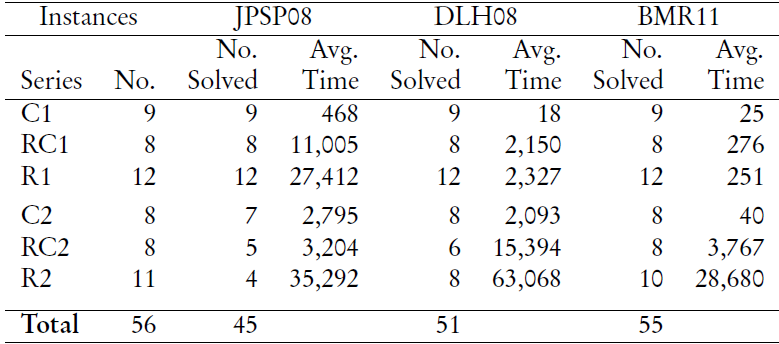
\includegraphics[scale=0.8]{figuras/rme.PNG}
\label{rme}
\caption{Resultados para métodos exatos}
\end{figure}

Para cada série de casos de 100 clientes, na Tabela de resultados obtidos por três algoritmos exatos , \cite{jepsen13},\cite{desaulniers14}, e \cite{baldacci11}, abreviado por JSPS08, DLH08, e BMR11. Nesta tabela, as duas primeiras colunas indicam a série de instância e o número de instâncias que ele contém. Para cada série e cada algoritmo, informa o número de casos que foram resolvidos para otimização (sem limite de tempo imposto) e o tempo médio em segundos para resolvê-los. Estes tempos são os relatados pelos autores e foram obtidos em computadores com características diferentes: P4 de 3,0 GHz para JSPS08, AMD Opteron de 2,6 GHz para DLH08 e IBM Intel Xeon X7350 a 2,93 GHz para BMR11. A última linha da Tabela proporciona o número total de ocorrências resolvidos por cada algoritmo.

Estes resultados mostram claramente que os exemplos na classe 2 são muito mais difíceis de resolver do que os exemplos da classe 1, porque janelas de tempo de longas aumentam o número de caminhos possíveis e o número de clientes por caminho viável, obtendo instâncias mais difíceis de resolver . Os resultados também mostram a evolução rápida dos algoritmos recentes. Antes do artigo de \cite{jepsen13}, apenas 35 dos 56 casos foram resolvidos. Com a introdução das desigualdades SR no algoritmo de \textit{Branch-and-Cut-and-Price}, \cite{jepsen13}. elevou este número para 43. Com busca tabu e gerador de colunas, o \textit{Branch-and-Cut-and-Price} de \cite{desaulniers14} resolveu 51 instancias . Com uma abordagem baseada no conjunto modelo de particionamento reduzida e contando com n \textit{g-paths} , \cite{baldacci11} resolveram todos os casos, exceto um, devido a uma falta de memória. Os tempos de computação são muito menores do que os anteriores, mas deve notar-se que o seu método requer um limite superior.

No futuro, podemos esperar para ver mais resultados computacionais para as instâncias de referência \cite{gehring09}, que estendem as definidos para casos que envolvem 200, 400, 600, 800, e 1000 clientes . Para o melhor de nosso conhecimento \cite{larsen00},\cite{braysy02} \cite{cook99}, \cite{kallehauge06} Relatam resolver alguns destes casos.
 
\section{Heurísticas}

Heurísticas são métodos de solução que muitas vezes podem encontrar soluções viáveis de boa qualidade de forma relativamente rápida. Segundo \cite{hillier05}, o procedimento normalmente é um algoritmo iterativo completo em que cada iteração envolve a condução de uma busca por uma nova solução que, eventualmente, poderia superar o melhor resultado encontrado previamente. Quando o algoritmo termina após um tempo razoável, a solução por ele fornecida é a melhor que foi encontrada durante qualquer iteração. No entanto, não há nenhuma garantia em relação à qualidade solução. Heurísticas são, assim, testados empiricamente e seu desempenho é julgado por seus resultados computacionais. Atualmente, a maioria das VRPs encontrados na indústria são resolvidas usando heurísticas por causa de sua velocidade e sua capacidade de lidar com grandes instâncias. A tradição dita que uma função objetivo hierárquica é usado quando heurísticas são aplicadas: a prioridade é minimizar o número de veículos utilizados e o segundo objetivo é minimizar o custo dos caminhos percorridos. Os algoritmos exatos que não consideram o número de veículos na função objetivo \cite{braysy05}.

As meta-heurísticas são uma classe de heurísticas mais recentes, que possuem como diferencial uma série de ferramentas que reduzem o risco de paradas prematuras em ótimos locais ainda distantes de um ótimo global. Geralmente estas ferramentas são componentes aleatórios inseridos durante a execução do algoritmo, que permitem que outras zonas de soluções sejam exploradas.

\subsection{Avaliação das Heurísticas }


A avaliação de qualquer método heurístico está sujeito à comparação de uma série de critérios que se relacionam com vários aspectos do desempenho do algoritmo. Exemplos de tais critérios são: tempo de execução, qualidade da solução, facilidade de implementação, robustez e flexibilidade \cite{cordeau12}. Uma vez que os métodos heurísticos são, concebidos para resolver problemas do mundo real, a flexibilidade é uma consideração importante. Um algoritmo deve ser capaz de lidar facilmente com as mudanças no modelo, as restrições e a função objetivo. Quanto à robustez, não deve ser excessivamente sensível às diferenças nas características do problema: uma heurística robusta não deve funcionar mal em qualquer instância. Além disso, um algoritmo deve ser capaz de produzir boas soluções cada vez que é aplicado a uma determinada instância. Isso deve ser destacado, pois qualquer heurística não é determinística e contém alguns componentes aleatórios, como valores de parâmetros escolhidos aleatoriamente. A saída de execuções separadas desses métodos não-determinísticos sobre o mesmo problema na prática nunca é a mesma. Isso torna difícil analisar e comparar resultados. Usando apenas os melhores resultados de uma heurística não-determinística, como muitas vezes é feito na literatura, pode criar uma imagem falsa de seu desempenho real. Assim, consideramos que os resultados médios baseados em execuções múltiplas em cada problema constituem uma base importante para a comparação de métodos não determinísticos. Além disso, também seria importante relatar o pior desempenho dos casos. Discussões extensas sobre esses assuntos podem ser encontradas em \cite{cordeau12}.



O tempo que uma heurística leva para produzir soluções de boa qualidade pode ser crucial ao escolher entre diferentes técnicas. Da mesma forma, a qualidade da solução final, medida pela função objetivo, é importante. Como a solução está próxima da solução ótima é uma medida padrão de qualidade ou, se a heurística é projetada para simplesmente produzir soluções viáveis, então a capacidade da heurística para fornecer essas soluções é importante.


Geralmente há um \textit{trade-off} entre o tempo de execução e a qualidade da solução - quanto maior o tempo que uma heurística é executada, melhor a qualidade da solução final. Um compromisso é necessário para que as soluções de boa qualidade que são produzidas em um período razoável de tempo. Basicamente, esse \textit{trade-off} entre tempo de execução e qualidade da solução pode ser visto em termos de uma otimização multi objetiva em que os dois objetivos são equilibrados. As medidas de desempenho para heurísticas podem ser plotadas em espaço bidimensional, com a primeira dimensão correspondente ao tempo de execução e A segunda para a qualidade da solução. Nesse espaço, pontos que não existem outros pontos com valores melhores em ambas as dimensões são considerados ótimos de Pareto; Eles definem compromissos efetivos entre os objetivos. \cite{russell94} e \cite{braysy05} . A escolha entre diferentes abordagens heurísticas produzindo resultados ótimos de Pareto depende das preferências do tomador de decisão e da situação em questão.


O método mais comum para avaliar a qualidade da solução de um algoritmo heurístico é a análise empírica. Em geral, a análise empírica envolve o teste da heurística em uma ampla gama de instâncias de problema para ter uma ideia do desempenho geral. Para se chegar a conclusões que tenham significado num sentido estatístico, o desenho experimental deve idealmente ser usado em diferentes níveis dos vários parâmetros do algoritmo e os resultados comparados por técnicas apropriadas.


Dificuldades enfrentadas especialmente no contexto PRVJT são que muitas vezes apenas os melhores resultados obtidos durante todo o estudo computacional são relatados. Além disso, em alguns casos os autores não relatam o número de execuções ou tempo de CPU necessário para obter os resultados relatados. Nestes casos é impossível concluir qualquer coisa sobre a eficiência dos métodos, ou comparar estes métodos com outras abordagens. A única base adequada para a comparação destes métodos seriam soluções ótimas, uma vez que se houver tempo suficiente disponível, é sempre preferível resolver os problemas com a optimização utilizando métodos exatos. Para ser capaz de chegar a conclusões apropriadas, além do número de execuções e consumo de tempo, deve-se responder a perguntas como quais são os limites do algoritmo dado, ou seja, quão bons são os melhores resultados que podem ser obtidos usando a abordagem particular , E como uma boa solução pode ser obtida em uma determinada quantidade de tempo. Em outras palavras, deve-se relatar resultados obtidos usando diferentes tempos de computação e observar quanto tempo é necessário para obter resultados de uma determinada qualidade. Além disso, na nossa opinião, os números que descrevem a relação entre a qualidade da solução e o tempo de computação facilitariam muito a análise. \cite{taillard01} discute extensivamente esta questão e propõe relatar um esforço computacional absoluto, como o número de iterações em vez de computar tempos e usar diagramas de probabilidade baseados em testes estatísticos repetidos de Mann-Whitney. Obviamente, tal abordagem não é possível quando se confia em resultados previamente publicados como fazemos aqui.




Os resultados são geralmente classificados de acordo com uma função objetivo hierárquica, onde o número de veículos é considerado o objetivo primário, e para o mesmo número de veículos, o objetivo secundário é muitas vezes a distância total percorrida ou a duração total das rotas. Portanto, uma solução que requer menos rotas é sempre considerada melhor do que uma solução com mais rotas, independentemente da distância total percorrida. De acordo com \cite{braysy01}, esses dois objetivos são muitas vezes conflitantes, o que significa que a redução no número de veículos frequentemente causa aumento na distância total percorrida. Assim, uma melhor solução em termos de distância total pode ser obtida aumentando o número de rotas. Alguns outros artigos relatam achados semelhantes, ver, por exemplo,\cite{caseau99}
 
 
\subsection{Heurísticas Para Construção de Rotas }


Heurísticas para construção de rotas seleciona nós (ou arcos) sequencialmente até que uma solução viável tenha sido criada. Os nós são escolhidos com base em algum critério de minimização de custos, muitas vezes sujeitos à restrição de que a seleção não cria uma violação da capacidade do veículo ou restrições de janela de tempo. Métodos sequenciais construir uma rota de cada vez, enquanto que os métodos paralelos construir várias rotas simultaneamente.



\cite{solomon87} propõe um esquema denominado rota-primeiro cluster-segundo usando uma heurística \textit{Giant-Tour}. Primeiro, os clientes são agendados em um \textit{Giant-Tour} e, em seguida, este \textit{tour} é dividido em um número de rotas menores. Um \textit{Giant-Tour} inicial poderia, por exemplo, ser gerado como um caixeiro viajante sem considerar as restrições de capacidade e tempo.


\cite{solomon87} descreve várias heurísticas para o PRVJT. Um dos métodos é uma extensão da heurística de poupança de Clarke e Wright (1964). O método de poupança, originalmente desenvolvido para a VRP clássica, é provavelmente a heurística de construção de rotas mais conhecida. Começa com uma solução em que cada cliente é fornecido individualmente por uma rota separada. Combinando as duas rotas que servem respectivamente os clientes i e j resulta em uma economia de custos de $ S_\gamma = d_{i0} + d_{0j} -d_\gamma $ Clarke e Wright (1964) selecionam o arco (i, j) ligando Clientes i e j com máximo $ S_ {ij} $ sujeitos à exigência de que a rota combinada seja viável. Com esta convenção, a operação de combinação de rotas é aplicada iterativamente. Ao combinar rotas, pode simultaneamente formar rotas parciais para todos os veículos ou adicionar sequencialmente clientes a uma determinada rota até que o veículo esteja totalmente carregado. Para ter em conta a proximidade espacial e temporal dos clientes, a \cite{solomon87} estabelece um limite para o tempo de espera da rota. 


A segunda heurística, uma vizinha mais próxima do tempo, inicia cada rota encontrando um cliente não roteado mais próximo do depósito. Em cada iteração subsequente, a busca heurística para o cliente mais próximo do último cliente adicionado na rota e adiciona-lo no final da rota. Uma nova rota é iniciada sempre que a pesquisa não consegue encontrar um local de inserção viável, a menos que não haja mais clientes não roteados. A métrica usada para medir a proximidade de qualquer par de clientes tenta explicar a proximidade geográfica e temporal dos clientes. A métrica usada para medir a proximidade de qualquer par de clientes tenta explicar a proximidade geográfica e temporal dos clientes.


A mais bem sucedida das três heurísticas de inserção sequencial propostas é chamada I1. Inicialmente, uma rota é inicializada com um cliente "semente" e os clientes não roteados restantes são adicionados a esta rota até que ela esteja cheia em relação ao horizonte de agendamento e / ou restrição de capacidade. Se os clientes não roteados permanecerem, as inicializações e os procedimentos de inserção serão repetidos até que todos os clientes sejam atendidos. Os clientes de semente são selecionados encontrando o cliente geograficamente mais distante não roteado em relação ao depósito ou o cliente não roteado com o menor tempo de início permitido para o serviço.


\section{Busca Local}

Um conceito central na maioria das heurísticas de sucesso para o PRVJT é a de busca local. Algoritmos de busca local são baseados em vizinhanças . Seja $\theta$ um conjunto de soluções viáveis para uma determinada instância PRVJT, e deixe c: $\theta \to$ R ser uma função que mapeia a partir de uma solução para o custo para esta solução. O conjunto $\theta$ é finito, mas muitas vezes é extremamente grande. Desde o PRVJT é um problema de minimização, o nosso objectivo é encontrar uma solução s* para o qual c(s*) $ \leq $c(s) para todo s $\in \theta$ . No entanto, com a heurística, estamos dispostos a se contentar com uma solução que pode ser ligeiramente inferior ao s*.

 
 Seja P($\theta$) o conjunto de subconjuntos de soluções em ($\theta$). Definimos uma função de vizinhança como uma função N:$\theta \to $ P($\theta$) P(S) que mapeia a partir de uma solução de s para um subconjunto de soluções de N(s). Este subconjunto é chamado o vizinho de s. Uma solução s é dito ser localmente ótima ou uma condição local no que diz respeito a uma vizinhança N(s) se c(s) $ \leq $ C($s^i$) de todos $s^i$ $ \in $ N(s). Com estas definições, podemos descrever um algoritmo decida acentuada(\textit{steepest descent}) (veja Algoritmo 3.1). O algoritmo leva uma solução s inicial como entrada. Em cada iteração, ele encontra a melhor solução $s^i$ na vizinhança N(s) da solução corrente s (linha 4). Se $s^i$ é melhor do que s (linha 5)
 
\begin{figure}[ht!]
\centering
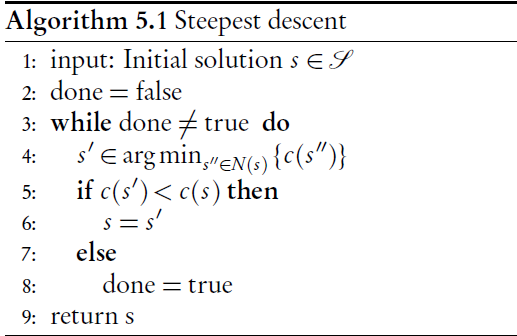
\includegraphics[scale=0.8]{figuras/alg-1.PNG}
\label{alg-1}
\caption{algoritmo \textit{steepest descent}}
\end{figure}

em seguida,$s^i$ substitui s como a solução atual (linha 6). Linhas 3-8 são repetidos enquanto $s^i$ melhorar a solução. Quando o loop parar, o algoritmo retorna s como a melhor solução encontrada. O algoritmo é chamado um algoritmo de descida acentuada, porque sempre escolhe a melhor solução na vizinhança atual.

Em geral,grandes vizinhanças conduzem a melhores soluções, quando as vizinhanças são utilizados, por exemplo, num algoritmo de descida mais acentuada. A desvantagem de grandes vizinhanças é que a avaliação de todas as soluções é mais demorada. Analisamos uma série de vizinhos que foram utilizados nas heurísticas PRVJT mais bem sucedidos. Classificamos esses vizinhos em duas categorias: vizinhos tradicionais e grandes. A primeira categoria engloba os vizinhos, cujo tamanho está crescendo polinomialmente com n de uma forma controlada de tal modo que todas as soluções na vizinhança podem ser avaliada por enumeração explícita.Vizinhos de tamanho cujo crescimento é tão rápida que não pode ser pesquisado explicitamente , e vizinhos cujo tamanho está a crescer exponencialmente \cite{ahuja00}. 

\subsection{2-opt}

Contém soluções obtidas através da remoção de dois arcos de uma rota e substituí-los por outros dois arcos para reconectar o percurso, ao alterar a orientação do subcaminhos que não contém o depósito. Na figura a praça representa o depósito e os círculos são clientes. Os arcos tracejadas correspondem a subcaminhos em G (ver Secção 3.2), envolvendo um ou vários arcos, enquanto que cada arco sólida corresponde a um único arco em G. Observe que alterar a orientação do subcaminhos (i + 1,.,.,. j + 1) pode ser problemática devido às janelas de tempo.


\subsection{Or-opt}

 Cada solução no vizinho or-opt é definido pela relocação de um subcaminho (i + 1,..., J) para uma posição diferente na rota. A orientação do subcaminhos realocado é preservada. O movimento é realizado através da remoção de arcos (i, i + 1), (j, j + 1), e (k, k + 1) e substituindo-os pelos arcos (i, j + 1), (k, i + 1 ), e (j, k + 1). Normalmente, o vizinho é reduzido, considerando apenas subcaminhos contendo um número limitado de clientes ou tentando apenas inserções que estão perto de sua posição original. \cite{braysy05}. 

\begin{figure}[ht!]
\centering
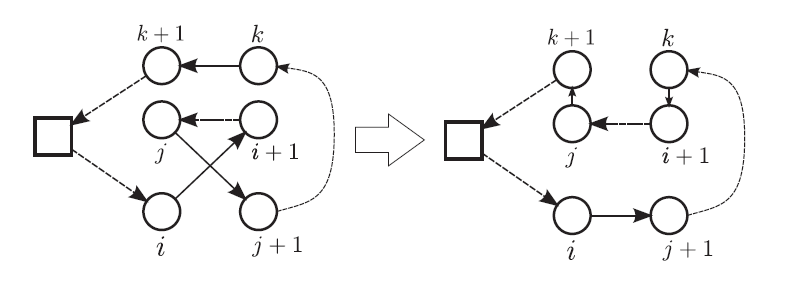
\includegraphics[scale=0.7]{figuras/opt-2.PNG}
\label{opt-2}
\caption{Or-opt}
\end{figure}

\subsection{2-opt*}

 O 2-opt* é definido de forma semelhante ao 2-opt , mas as suas soluções são derivadas modificando duas rotas em vez de uma. Dois arcos, (i, i + 1) e (j, j + 1), a partir de duas rotas distintas são removidos, e as rotas são restabelecida através da inserção dos arcos (i, j+1) e (j, i+1) . O efeito é que as extremidades das duas rotas são trocados. O 2-opt* não altera a orientação dos subcaminhos, em oposição ao 2-opt.

\begin{figure}[ht!]
\centering
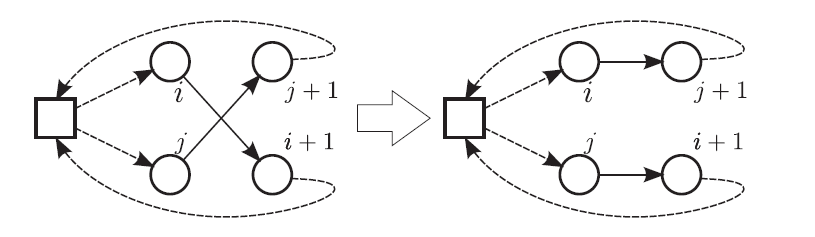
\includegraphics[scale=0.7]{figuras/opt-3.PNG}
\label{opt-3}
\caption{2-opt*}
\end{figure}

\subsection{\textit{Cross Exchange}}

 No vizinho de intercâmbio, dois subcaminhos são selecionados e as suas posições são trocadas. Isto é feito através da remoção de quatro arcos (i, i + 1), (j, j + 1), (k, k + 1), e (L, L + 1) e substituindo-os pelos arcos (I, K + 1), (L, J + 1), (K, i + 1), e (j, l + 1). O tamanho da vizinhança de troca cruzada é tipicamente reduzida por considerar apenas subcaminhos que contêm um número limitado de clientes. Notamos que \textit{Cross Exchange} pode ser utilizado de forma intra-percurso onde os subcaminhos para ser trocado pertencem à mesma via.
 
\begin{figure}[ht!]
\centering
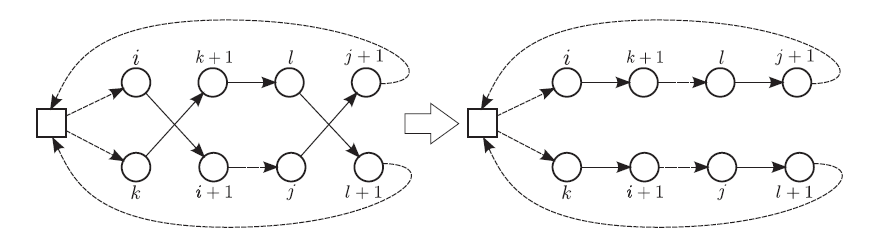
\includegraphics[scale=0.7]{figuras/opt-4.PNG}
\label{opt-4}
\caption{Cross Exchange}
\end{figure}
 
\subsection{Realocação de Caminho}
 No caminho de realocação , as soluções são obtidas através da relocação de um subcaminho de uma rota para outra. Isto é feito através da remoção de três arcos (i, i + 1), (j, j + 1), e (k, k + 1) e substituindo-os pelos arcos (i, j +1), (J, K + 1), e (k, i + 1). Esta zona pode ser visto como um caso especial de vizinhança de troca cruzada, se permitirmos que um subcaminhos vazio no último vizinhança. O comprimento do subcaminhos realocada é tipicamente limitado, e algumas implementações permitir que o subcaminhos de ser invertida quando é reinserido. 
 
\begin{figure}[ht!]
\centering
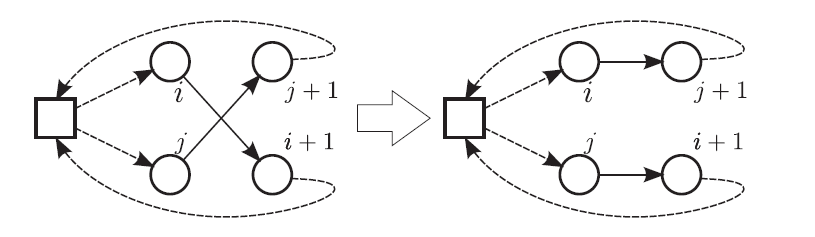
\includegraphics[scale=0.7]{figuras/opt-3.PNG}
\label{opt-5}
\caption{Realocação de Caminho}
\end{figure}
 
 
 \subsection{Técnicas de aumento de velocidade}
 
 Em busca local, é importante para implementar a avaliação vizinho de forma eficiente, a fim de procurar tantas soluções quanto possível dentro do tempo previsto para a pesquisa. Cada movimento nos vizinhos mencionados acima podem ser avaliadas em tempo constante utilizando as técnicas descritas em \cite{kindervater97}, mas para grandes instâncias isso pode não ser suficiente. Por isso, é comum a truncar a busca na vizinhança de uma maneira heurística de tal forma que alguns movimentos que não parecem promissores não são avaliados. Isto pode ser feito considerando-se apenas movimentos que ligam os clientes próximos; considerações de janela de tempo pode também ser tida em conta. Dois exemplos de tal filtragem pode ser encontrado em \cite{uno00} , \cite{nagata10}.
 
 \cite{daniel14} introduziu busca sequencial para o PRVJT. busca sequencial é capaz de acelerar a busca local usando a filtragem exato onde grandes subconjuntos dos movimentos possíveis pode ser ignorada com base em considerações de custo. resultados computacionais mostram speedups impressionantes para instâncias PRVJT em grande escala. pesquisa sequencial tem, com o melhor de nosso conhecimento, não foi ainda utilizada nos PRVJT mais bem sucedidos.
 
 
 \subsection{Permitindo Soluções inviáveis}
 
Ao projetar meta-heurísticas para a PRVJT, deve-se decidir se soluções inviáveis deve ser permitido durante a pesquisa. Quando permitido, eles são tipicamente penalizada na função objetivo por um ou mais termos que visam reduzir inviabilidade. Permitindo soluções inviáveis torna mais fácil de manobrar no espaço de solução, fornecendo atalhos entre as áreas de soluções de alta qualidade. Por outro lado, aumenta a complexidade do algoritmo: avaliação do objetivo pode ser mais difícil, parâmetros de penalidade deve ser ajustado (potencialmente de um modo adaptativo), e deve-se assegurar que as soluções viáveis são visitadas pelo menos de vez em quando. Apesar destes inconvenientes, permitindo soluções inviáveis parece ser uma ferramenta importante para encontrar soluções de alta qualidade.
 
 

Nas meta-heurísticas atuais são permitidos três tipos de soluções inviáveis : janela de tempo, capacidade do veículo, e as violações de atendimento ao cliente. O último tipo ocorre quando alguns clientes não são visitados. É o tipo mais comum nos algoritmos que minimizam o número de veículos utilizados. violações de janelas e de capacidade de tempo são normalmente autorizados juntos e levar a um c(s) função objetivo penalizada.

Em que c(s) é a função de objetivo padrão e q(s) (resp., w(s)) mede a capacidade total (resp., tempo-janela) violação sobre todas as rotas. E são parâmetros que são geralmente ajustados durante a pesquisa, reagindo ao desempenho do algoritmo. Um bom exemplo de como a parâmetros e pode gestão é dado em \cite{cordeau01}.


Violação de uma janela de tempo ao longo de uma rota r = (... $v_0$ = 0, $v_1$, $v_2$,..., $v_k$, $v_{k + 1}$ = n + 1) é calculada diretamente: o início do tempo de serviço $T_{V_{I}}$ no vértice $v_i$ é calculado como 


e a violação total é de $ \sum_{k + 1}^{i = 1}$max{0, $T_{v_{i}}$ - $b_{v_{i}}$}. A desvantagem deste procedimento é que a avaliação de um movimento nos vizinhos já não pode ser realizada em tempo constante. Em vez disso, \cite{nagata10} propôs um início artificial do avaliação do tempo de serviço que se move do início para o fim da janela de tempo sempre que for violada.



Violação da janela de tempo é dada por $ \sum_{k + 1}^{i = 1}$max{0, $T_{v_{i}}^i$ - $b_{v_{i}}$}, uma fórmula que ainda captura violações de janela de tempo e faz com que seja possível avaliar em tempo constante um único movimento nos vizinhos \cite{gendreau10}.


\subsection{Minimizar o Numero de Veículos Usados }

É tipicamente executada em duas fases, onde uma primeira procura encontrar o menor número de veículos necessários e, em seguida, mantém este número fixo enquanto minimiza o custo total da viagem. Se a heurística permite visitar soluções inviáveis, então pode-se selecionar um número de veículos m e criar uma solução (possivelmente inviável) com esse número de veículos. Em seguida, uma pesquisa é realizada com o objetivo de encontrar uma solução viável. Se a pesquisa for bem sucedida, o número de veículos é reduzida no excluindo uma rota completa antes de repetir a busca. Caso contrário, o número de veículos é aumentado no e a pesquisa é repetida ,se ainda não houver soluções viáveis encontradas . Usando um limite inferior calculado sobre o número de veículos, é possível parar a busca de um menor número de veículos, quando o limite inferior é atendido. A pesquisa para o número mínimo de veículos também pode ser abortado quando um esforço suficiente foi investido. \cite{nagata10} criaram um do procedimento rota minimização mais eficaz.


\subsection{Pesquisa Caminho Único} 

Parte de uma única solução, algoritmos de busca caminho único gerar uma sequência de soluções que podem ser vistos como uma trajetória através do espaço de solução. Em cada iteração, apenas a solução de corrente é utilizada para determinar a próxima.
 
\cite{hashimoto_iterated_2008} desenvolveram um algoritmo de busca local iterado por uma variante do PRVJT onde as janelas de tempo são representados por funções de penalidade linear convexa, por partes. O PRVJT é um caso especial deste problema quando a função de penalidade é definida de forma adequada (penalidade infinita fora da região viável). Por causa das funções de penalidade, é não-trivial para determinar o melhor momento de partida possível para uma determinada rota. Esse problema é chamado o \textit{Optimal Start Time Problem} (OSTP). Os autores apresentam um algoritmo de programação dinâmica para a OSTP e descrever como o algoritmo de programação dinâmica pode ser acelerado no algoritmo de busca local. Note que o OSTP foi previamente estudado por \cite{Desrochers88}, que considerou funções de penalidade convexas arbitrárias.


 
\cite{hashimoto_iterated_2008} propôs um algoritmo de busca local iterado para uma PRVJT dependente do tempo com janelas de tempo suaves por busca local iterativa. Como antes, é uma tarefa não trivial para determinar o tempo de partida de uma rota ótima. Quando um ótimo local é encontrado, a solução atual é perturbado pela aplicação de um único movimento de troca aleatório para a solução. O algoritmo é usado para resolver instâncias PRVJT, permitindo violações janela de tempo e ajustar penalidades de forma adequada.
 
 
\cite{cordeau2011} introduziu um algoritmo de busca local iterado que se baseia na versão atualizada do algoritmo de busca tabu de \cite{cordeau04}, como o algoritmo de busca local. O algoritmo de busca tabu permite soluções que são inviáveis no que diz respeito às duas janelas de tempo e capacidade do veículo. Ele usa uma vizinhança simples, baseada na realocação do cliente. O passo perturbação é inspirado pelo LNS e consiste em remover um conjunto de clientes e reinserindo-os na ordem aleatória. Cada cliente é reinserido na rota utilizando uma política \textit{cheapest-insertion}.

\begin{figure}[ht!]
	\centering
	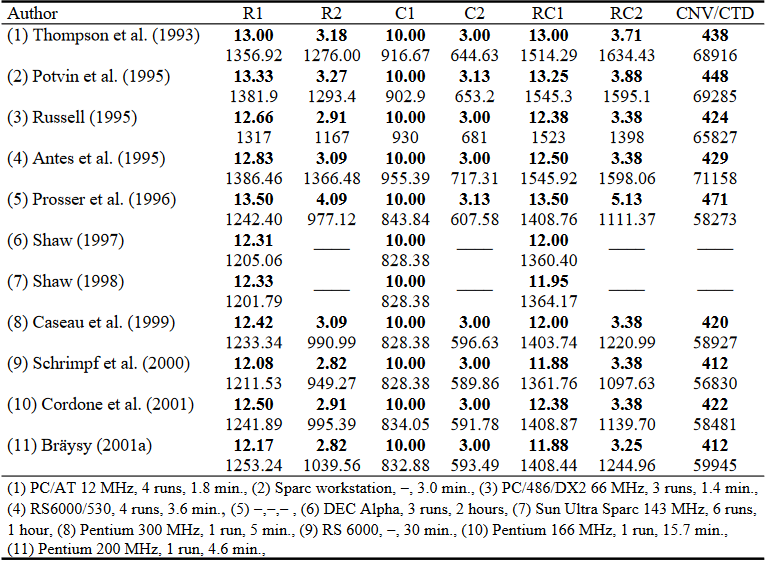
\includegraphics[scale=0.7]{figuras/rbl.PNG}
	\label{rbl}
	\caption{Resultados obtidos com as heurísticas de busca local}
\end{figure}


\section{Large Neighborhood Search}


 O LNS heurística original por \cite{shaw98} já resolveu o PRVJT com bons resultados no conjunto reduzido de casos, mas foi só com o trabalho de \cite{bent04} que a capacidade do método para a obtenção de boas soluções para o PRVJT foi totalmente revelado.A pesquisa funciona escolhendo de forma aleatória um conjunto de visitas de clientes. Os clientes selecionados são removidos da programação e, em seguida, reinseridos com o custo ótimo. Para criar a oportunidade para o intercâmbio de visitas de cliente entre rotas, as visitas removidas são escolhidas de modo que estejam relacionadas. Aqui, o termo relacionado refere-se a clientes que estão geograficamente próximos um do outro, servidos pelo mesmo veículo, têm uma procura semelhante de mercadorias e tempos de início semelhantes para o serviço. Um ramo e método ligado acoplado com a Programação de Restrição é então usado para reprogramar visitas removidas. Na solução inicial, cada cliente é servido por um veículo separado. Devido aos elevados requisitos computacionais, esta abordagem só pode ser aplicada a problemas em que o número de clientes por rota é relativamente baixo.
 
 
\section{Busca Tabu}
 
A meta-heurística Busca Tabu (BT) é uma técnica que segue os princípios gerais de Inteligência Artificial (IA) e é utilizada para guiar o procedimento de busca local na busca do ótimo do problema. BT toma da IA o conceito de memória e a implementa mediante estruturas simples com o objetivo de conduzir a busca considerando o histórico da mesma. O procedimento trata de extrair informação do passado recente e atuar em função dessa informação. Neste sentido pode-se dizer que existe um certo aprendizado e que a busca é inteligente. 


Busca Tabu tem suas raízes na década de 60, mas a forma como hoje é apresentada foi proposta por \cite{glover97}. BT é uma abordagem plenamente aceita para o tratamento de problemas de otimização combinatória e tem se mostrado como uma técnica muito promissora através de inúmeras aplicações bem sucedidas. 

O método é uma técnica iterativa que explora o conjunto de soluções de um problema, movimentando-se de uma solução S para outra solução S*, numa determinada vizinhança N(S) de S. Esses movimentos são executados com o intuito de alcançar eficientemente uma solução qualificada como boa, que pode ser ótima ou próxima da ótima. Ao contrário de um algoritmo simples de descida, BT aceita soluções S*piores que S, evitando assim o problema de ótimo local, fazendo uso de uma estrutura de memória capaz de suportar e até encorajar uma busca não monotonicamente decrescente (em problemas de minimização). BT percorre o espaço de busca, analisando os movimentos através de regras determinísticas. Quando BT aceita movimentos que pioram o valor da função objetivo, podem ocorrer ciclos, isto é, o retorno a soluções já visitadas. Para evitar que ciclagens se estabeleçam, BT armazena os atributos das soluções já pesquisadas em uma lista chamada lista tabu. Os atributos armazenados são muitas vezes usados para impor condições, chamadas restrições tabu, que impedem a escolha de movimentos indesejáveis. Um movimento é chamado tabu se conduz a soluções cujos atributos estão contidos na lista tabu ou satisfazem restrições tabu. Após um determinado número de iterações a lista tabu é alterada. 


Uma estrutura de geração de vizinhança de boa qualidade é fundamental para o sucesso da técnica. Se um movimento provoca uma variação muito pequena na função objetivo, é razoável supor que a busca por boas trajetórias para escapar de um mínimo local será problemática. Por outro lado, se essa amplitude é grande, certamente haverá dificuldades para encontrar um mínimo local cuja qualidade seja próxima do mínimo global. 


Existem alguns refinamentos que podem ser implementados no procedimento padrão de BT de forma a torná-lo mais eficiente. Esses refinamentos tentam introduzir mais inteligência no processo de busca. Um deles se refere ao tamanho da lista tabu, que varia de acordo com o problema em estudo. O tamanho da lista depende também das restrições tabu empregadas. Em geral, restrições fortes implicam em listas pequenas. Uma maneira de identificar-se o tamanho da lista apropriada é simplesmente observar a ocorrência de ciclos (listas muito pequenas) e a deterioração da qualidade da solução (listas muito grandes). A melhor lista certamente estará entre esses extremos. Outro aprimoramento que se relaciona com o tamanho da vizinhança é a construção de uma lista de candidatos. Um exame completo de vizinhança geralmente proporciona soluções de boa qualidade, porém pode consumir muito tempo computacional. Por essa razão é importante a utilização de estratégias que isolam regiões da vizinhança contendo movimentos desejáveis e os colocam em uma lista de candidatos. Existem estudos sobre técnicas de decomposição de vizinhança, construção de listas de movimentos promissores, listas dos atributos preferidos e muitos outros. 


Uma implementação bastante atraente consiste na variação da penalidade imposta à função objetivo para destruir a estrutura de otimalidade local da qual se deseja escapar. A variação da penalidade é exemplo de um procedimento conhecido como oscilação estratégica , que representa uma das abordagens básicas de diversificação da busca tabu. A oscilação pode cruzar os limites e penetrar em regiões de inviabilidade ou somente se aproximar e recuar, sem transpor esses limites. Uma maneira simples de se implementar essa penalidade é alternar uma série de movimentos que melhoram a função objetivo com outra série de movimentos que a pioram. 
 

\section{Pesquisas em Populações}

Meta-heurísticas que são baseadas na ideia de manter uma pool de soluções, chamada de população, que evolui a cada iteração do processo de solução. Ao contrário de pesquisa única trajetória, novas soluções são derivados a partir de uma população de soluções que oferece diversidade em si. Abaixo, vamos examinar as recentes obras sobre o PRVJT baseados em algoritmos evolutivos religação e trajeto, duas famílias de heurísticas de busca populacional.
 

\subsection{Algoritmos evolutivos}

Algoritmos evolutivos combinam soluções da população atual para produzir uma nova população. O mais adaptado deles é então retido para atualizar a população. A meta-heurística de Algoritmos Genéticos (AG) foi introduzida por \cite{holland75} inspirado no processo observado da evolução natural dos seres vivos, tentando imitar os mecanismos de reprodução existentes na natureza. Os AG estabelecem uma analogia entre o conjunto de soluções de um problema e o conjunto de indivíduos de uma população, codificando a informação de cada solução num vetor chamado de cromossomo. Para isso se introduz uma função de avaliação dos cromossomos, isto é a função objetivo (função aptidão). Igualmente se introduz um mecanismo de seleção de tal modo que os cromossomos com melhor avaliação sejam escolhidos para que se reproduzam. 

Quando se trabalha com os AG tem-se que levar em consideração a necessidade de se integrar e implementar eficientemente duas ideias fundamentais: as representações simples como vetores das soluções do problema e a realização de transformações simples para modificar e melhorar essas soluções. Para implementar os AG tem-se que considerar vários elementos principais tais como: a representação do cromossomo, uma população inicial, a função que avalia o cromossomo, os critérios de seleção e eliminação do cromossomo, uma ou varias operações de recombinação ( crossover ), uma ou varias operações de mutação . 


Em geral a população inicial é gerada aleatoriamente. No entanto, ultimamente se estão utilizando métodos heurísticos para gerar soluções iniciais com boa qualidade. Neste caso é importante garantir a diversidade estrutural das soluções para evitar a convergência prematura. Em relação à avaliação dos cromossomos em geral utiliza-se o valor da função objetivo do problema. 

A operação da mutação mais simples e uma das mais utilizadas consiste em substituir com certa probabilidade o valor de um bit. O papel que cumpre a mutação é de introduzir um fator de diversificação, pois em determinadas ocasiões a convergência do procedimento a boas soluções pode ser prematura e ficar preso em ótimo locais. Outra forma de introduzir novos elementos numa população é combinar elementos tomados aleatoriamente sem considerar a função aptidão. 
 
\begin{figure}[ht!]
\centering
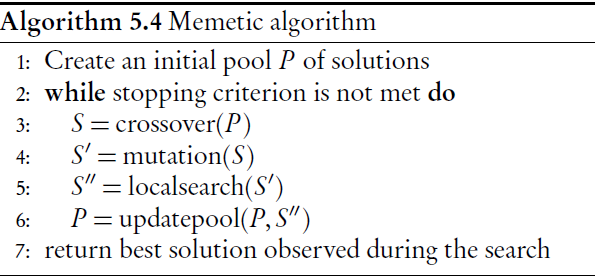
\includegraphics[scale=0.8]{figuras/alg-4.PNG}
\label{alg-4}
\caption{Algorítimos meméticos}
\end{figure}

 
Algoritmos meméticos hibridizam algoritmos genéticos com busca local e potencialmente algoritmos específicos de problemas. O tamanho da população inicial criada na linha 1 é, obviamente, um parâmetro importante. Linhas 2 a 6 constituem o ciclo principal do algoritmo que pode ser parado de acordo com vários critérios com base no número de iterações realizada, o tempo decorrido, ou uma medida da convergência. Na linha 3, novas soluções, formando conjunto S são construídos através da combinação de soluções existentes de P. Esta operação é chamado de crossover. Na linha 4, a mutação é aplicado a um subconjunto das soluções em C para criar um novo subconjunto de indivíduos $ S^{i} $, perturbando deste modo a definir prole. O passo de mutação não está incluído em todos os algoritmos meméticos. Na linha 3. a busca local é executado em cada solução prole em $ S^{i} $ para gerar um conjunto $ S^{ii} $ de soluções melhoradas. Às vezes, esta etapa de busca local é visto como uma operação de mutação. As soluções em $ S^{ii} $ são então usadas para atualizar a população P (linha 6). Uma maneira simples de efetuar esta atualização consiste em manter as melhores soluções $ \|P\| $ do conjunto P ($ S^{ii} $, mas um processo mais avançado é normalmente usado para favorecer a diversidade da população P. Um algoritmo genético clássico é obtido através da remoção da etapa de busca local (linha 5) no Algoritmo

 


Um dos Componentes vitais em algoritmos meméticos é o algoritmo \textit{crossover}. Abaixo damos uma visão geral dos métodos de crossover utilizados nos algoritmos evolutivos de maior sucesso para a PRVJT.
 


\subsection{\textit{Crossover} EAX}

 O algoritmo de \textit{crossover} EAX é baseado no algoritmo de \textit{crossover} forte para o TSP, que foi introduzido pela primeira vez por  \cite{nagata06} e tem sido a base dos melhores algoritmos evolucionários para o TSP.
 
 
\subsection{\textit{Crossover} OX}

OX crossover é um  crossover clássico para representações de soluções à baseadas em permutações \cite{falkenauer91}. Figura ilustra esse crossover para permutações dos números de 1 a 9. Um escolhe dois números aleatórios i e j e cria uma permutação para o individuo que vai ser gerado, copiando o pedaço de pai 1 a partir da posição i para j na posição i para j da prole. A parte restante da prole é encontrado copiando elementos de pai 2, respeitando a ordem de pai 2.
 
 
 
\begin{figure}[ht!]
\centering
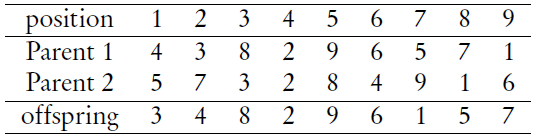
\includegraphics[scale=0.8]{figuras/ox-crossover.PNG}
\label{ox-crossover}
\caption{Ox \textit{crossover}}
\end{figure}
 
\subsection{Religação de Caminhos}



\cite{hashimoto08} desenvolveram um algoritmo de religação caminho para o PRVJT que funciona com um conjunto de soluções e permite soluções inviáveis que são penalizadas. Os pesos de penalização são controlados de forma adaptativa, dependendo se de viabilidade é fácil ou difícil de atingir. Em cada iteração exterior do algoritmo, as duas soluções A e B a partir da população são selecionados aleatoriamente. O algoritmo transforma A em B por uma série de 2-opt* e OR-opt movimentos. Isto gera uma série de soluções de entre as soluções A e B. No laço interno, algumas destas soluções são melhoradas usando vizinhos 2-opt*, intercâmbio, e Or-opt. Certas soluções gerados são adicionados à solução de população se melhorar a qualidade da população, tendo em conta inviabilidade total inviabilidade tempo, e inviabilidade capacidade.
 

\section{Considerando os Motoristas, com Múltiplos Veículos e Múltiplas Janelas}

O PRVJT com os regulamentos motorista leva em conta vários regulamentos referentes às horas de trabalho, pausas e descansos dos motoristas. Estes regulamentos estão aparecendo cada vez mais frequentemente em todo o mundo e podem variar de região para região. Para este problema, \cite{goel08} introduziram uma heurística LNS com base em operadores de pesquisa locais, \cite{prescott09} desenvolveram um método LNS com base na heurística de geração de colunas, e \cite{kok10} propuseram uma heurística de programação dinâmica. De acordo com os resultados computacionais relatados obtidos em instâncias envolvendo 100 clientes ao longo de um horizonte de uma semana, o algoritmo de \cite{prescott09}. supera os outros dois algoritmos.

O CVRP com o uso múltiplo de veículos é uma variante do CVRP clássica que permite atribuir várias rotas para o mesmo veículo ao longo de um horizonte de planejamento finito (por exemplo, o primeiro dia de trabalho) no contexto onde a disponibilidade do veículo, os custos de veículos fixo, ou tempo máximo de trabalho por veículo deve ser considerada. \cite{azi12} abordou o caso com janelas de tempo e projetado um método de solução de \textit{Branch-and-Price} exata. Eles resolveram instâncias com até 40 clientes.

\cite{doerner10} estudaram a VRP com várias janelas de tempo interdependentes em que podem ser exigidas a cada cliente a ser visitado várias vezes e o tempo decorrido entre duas visitas consecutivas não deve exceder o tempo máximo. Essa variante do PRVJT é inspirada por um pedido de transporte de sangue. Os autores desenvolveram um algoritmo exato e algoritmos heurísticos. Os seus resultados mostram que os algoritmos heurísticos encontrar soluções razoavelmente perto de soluções ótimas numa fracção de um segundo.

